\section{Landing legs} 
\label{ea:landing-legs}
Engineering analysis was conducted to evaluate four versus three landing legs. Reducing mass was essential to display functionality of the thrust mechanism. Reducing the number of landing legs would significantly decrease the mass, however it would lead to the rocket toppling for a smaller landing angle. This is largely due to four landing legs providing the rocket with a larger footprint (Figure \ref{figs:4ll}) than three landing legs (Figure \ref{figs:3ll}.


\begin{figure}[H]
\centering
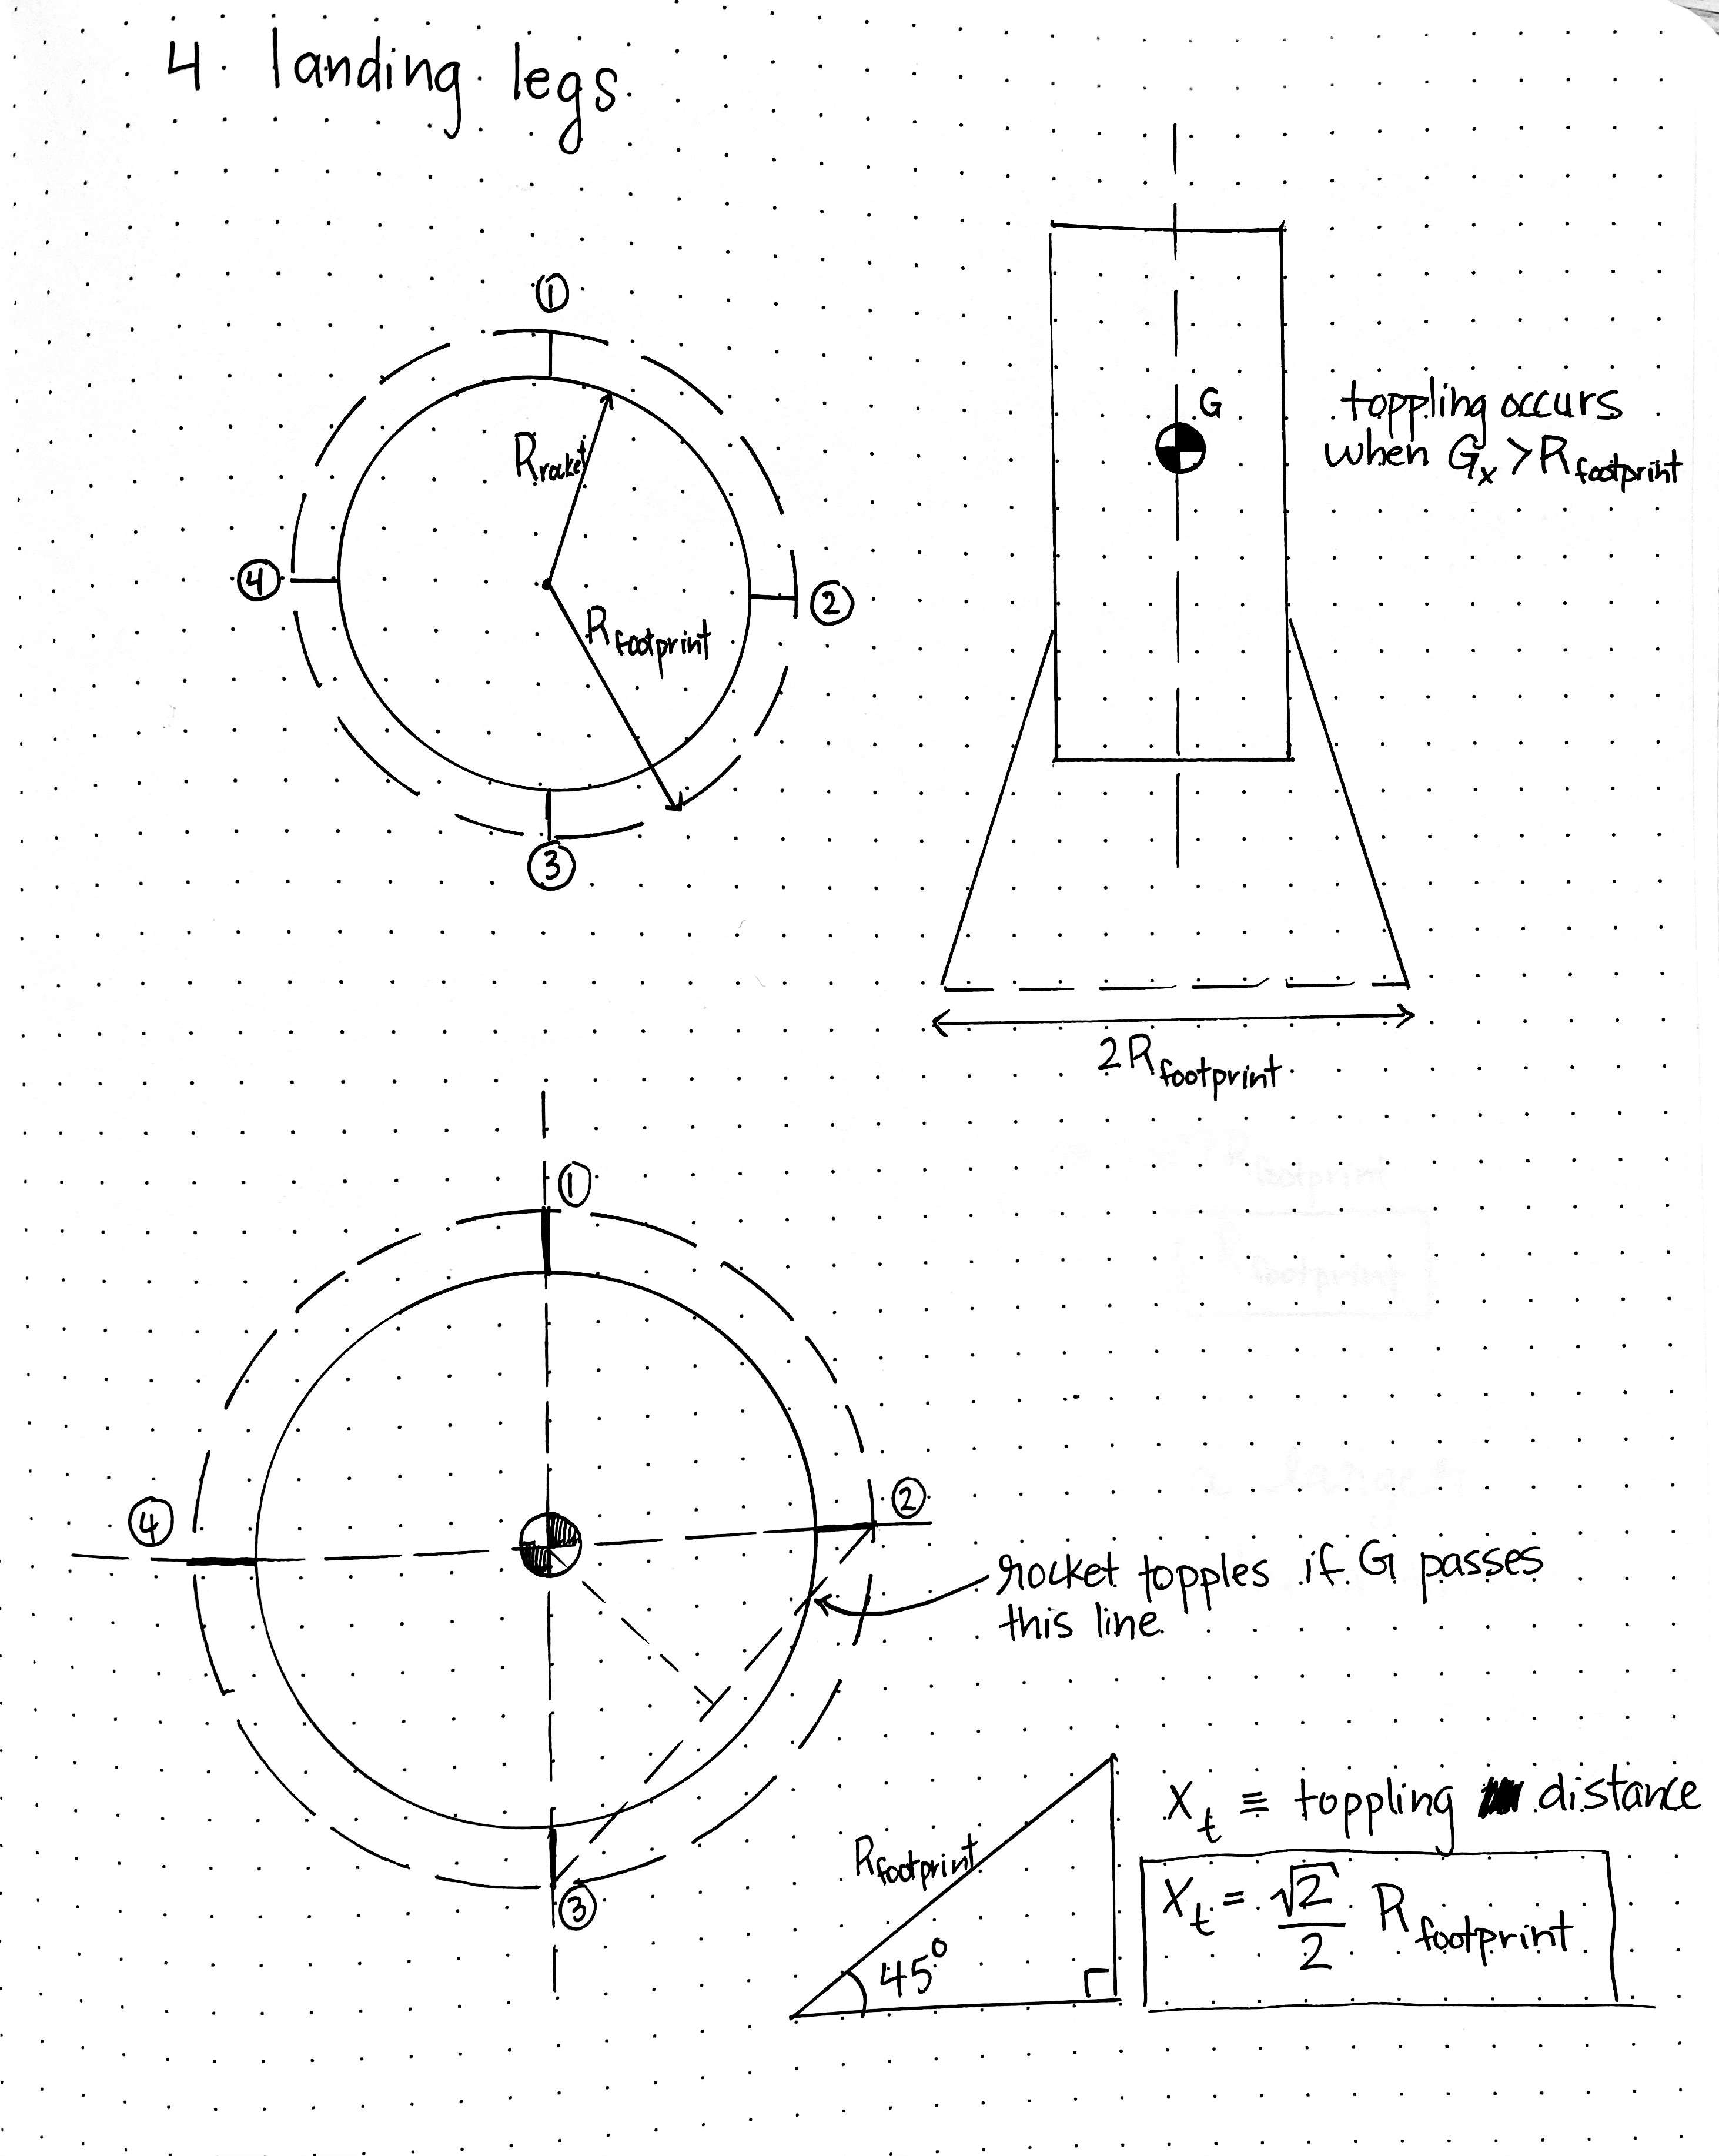
\includegraphics[scale=0.1]{src/figs/4landinglegsdrawing.jpeg}
\caption{Four landing legs analysis}
\label{figs:4ll}
\end{figure}

\begin{figure}
\centering
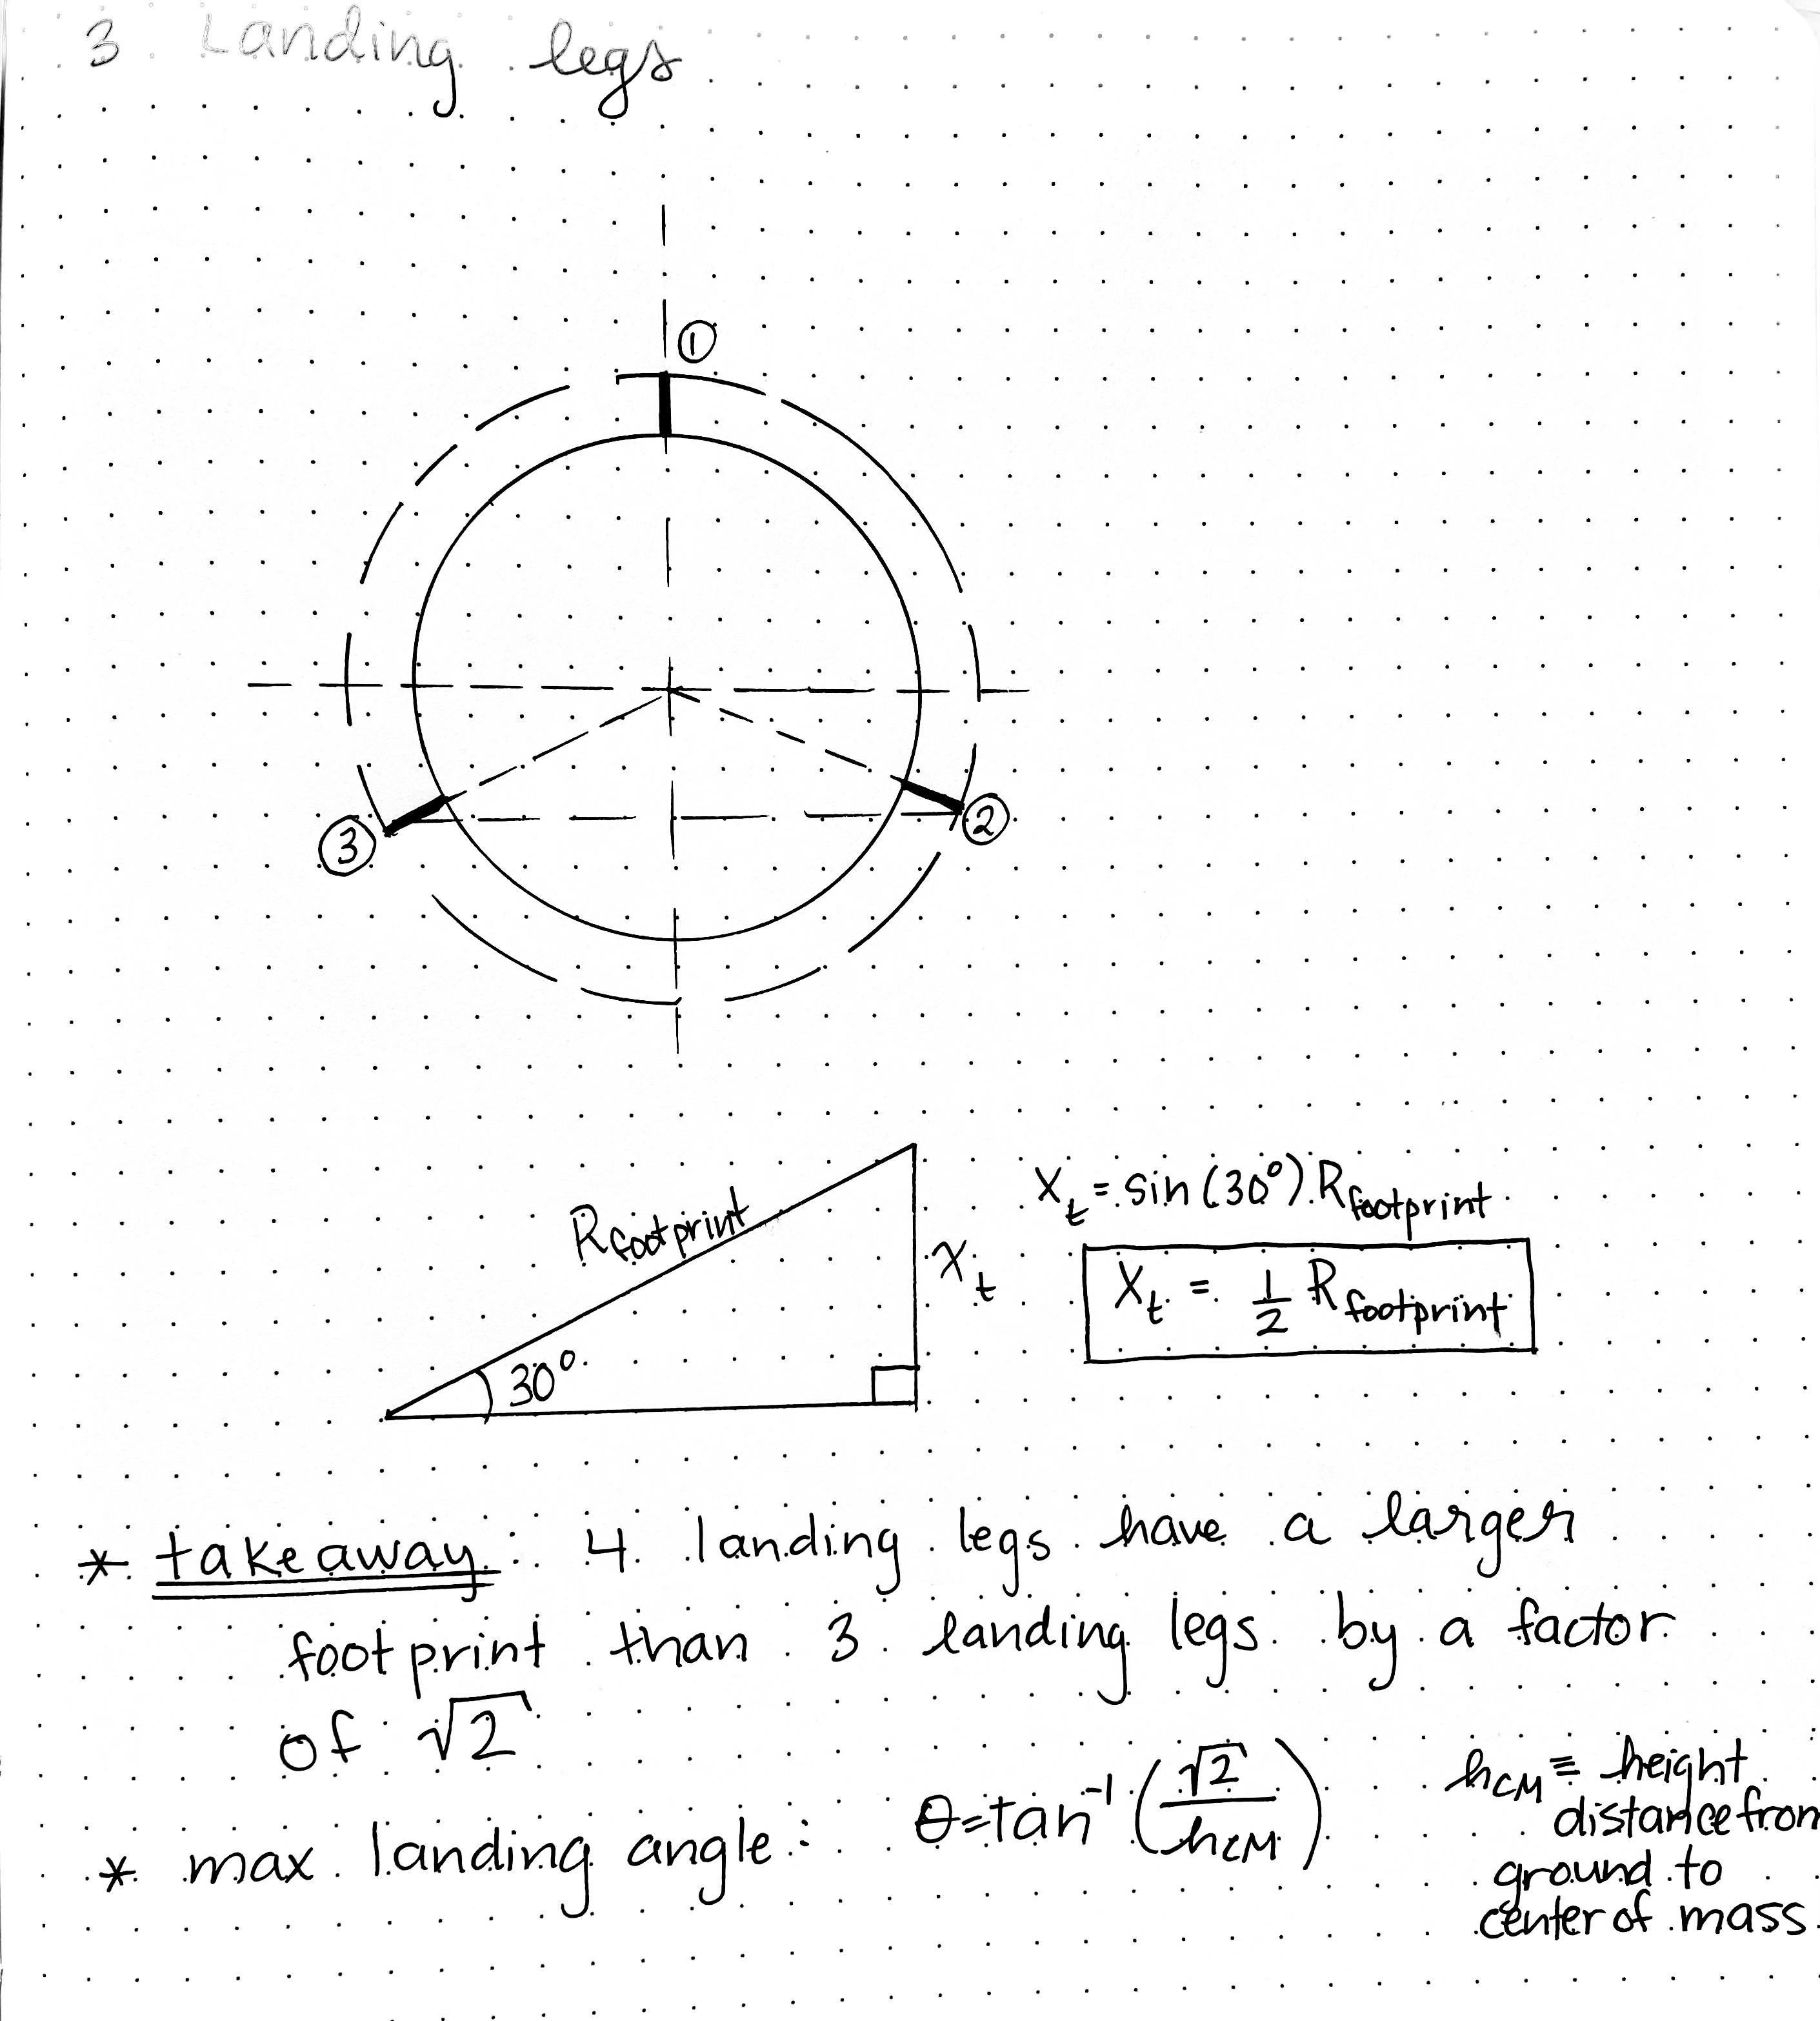
\includegraphics[scale=0.1]{src/figs/3landinglegsdrawing.jpeg}
\caption{Three landing legs analysis}
\label{figs:3ll}
\end{figure}

The main takeaway from these calculations is that four landing legs have a larger distance that the center of gravity can travel from its upright position. This means that toppling will not occur for a larger range of landing angles, namely up to $\theta = (tan^{-1}(\sqrt{2})/h_{cm})$. If $h_{cm}$ is estimated to be 15 inches, the difference in maximum angles between three versus four legs is 5.4 degrees. In the final design, the center of mass is 8.1 inches below the propeller blades in their deployed position leading to a difference of about 10 degrees. Minimizing mass is the most important to our needs because the rocket assembly will not be able to take off and land. Minimizing mass can also help the controlled orientation of the rocket with the rotors, so having that small grace distance with four landing legs is not worth the added stability. 



Determining an optimal leg angle was integral to meeting the needs of the rocket being structurally sound when under the landing load and its ability to land in a stable, upright position. A schematic of the primary and secondary struts along with the angles to be determined are shown below in Figures \ref{figs:aa}, \ref{figs:fp}. The purpose of these calculations is to find an angle that allows for a large enough footprint to stabilize the rocket body upon landing while minimizing leg stress and mass. Increasing $\alpha$ and decreasing $\beta$ leads to longer strut lengths and increased mass. To increase stability and mitigate accumulating mass, the angles were determined by force calculations with stability in mind. 

\begin{figure}[H]
\centering
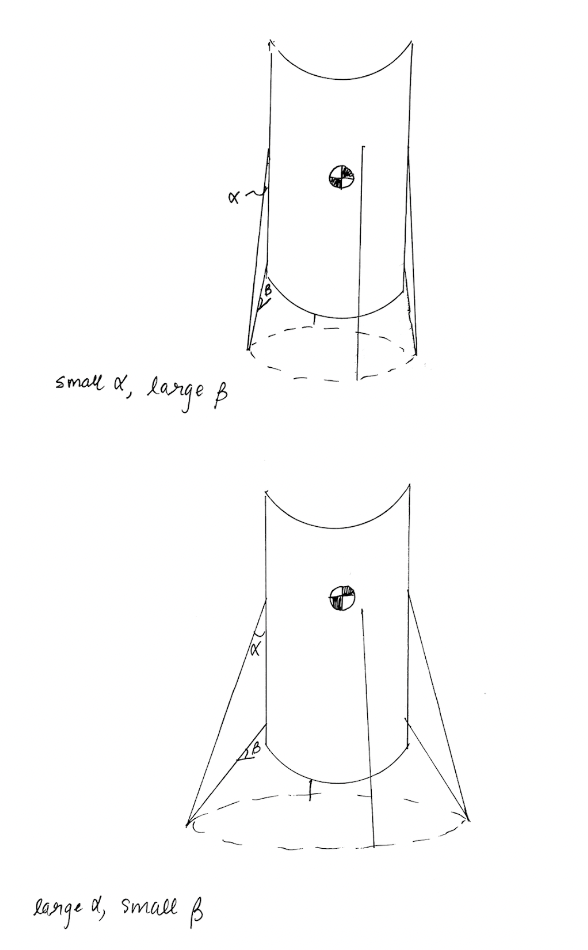
\includegraphics[scale=0.3]{src/figs/footprint.png}
\caption{Angle Analysis}
\label{figs:fp}
\end{figure}

\begin{figure}[H]
\centering
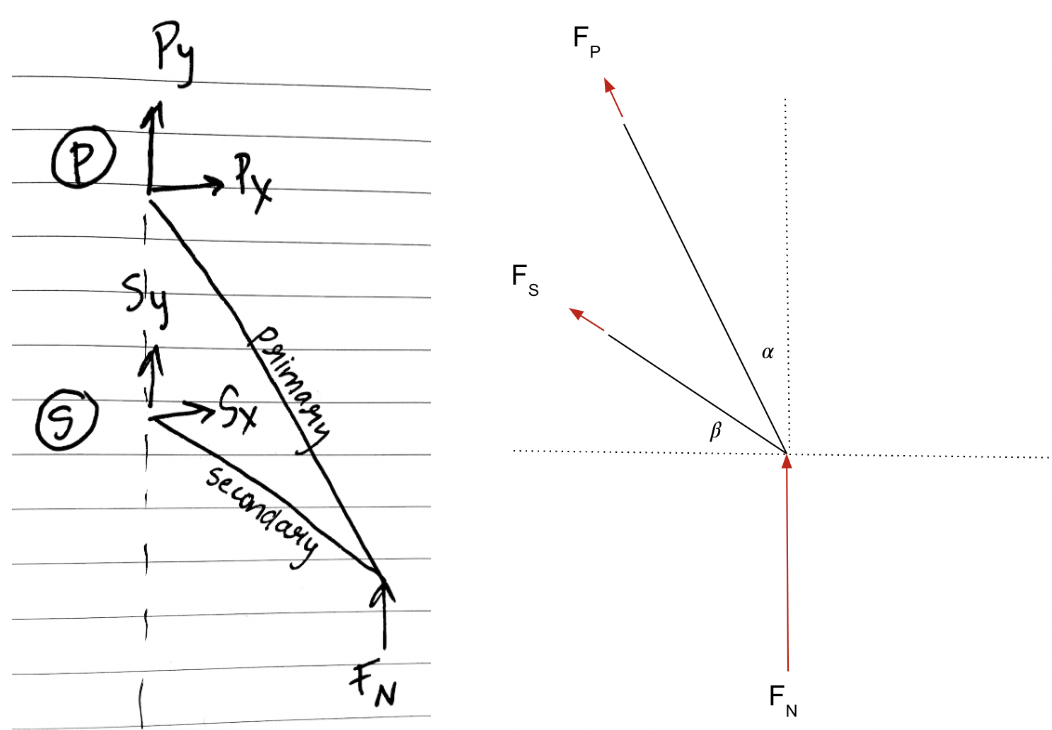
\includegraphics[scale=0.3]{src/figs/angleanalysis.png}
\caption{Angle Analysis}
\label{figs:aa}
\end{figure}

The free body diagram analysis yields the following equations [Figure \ref{figs:forceeqn}] with Fp representing the force in the primary strut and Fs representing the force in the secondary strut. 

\begin{figure}[H]
\centering
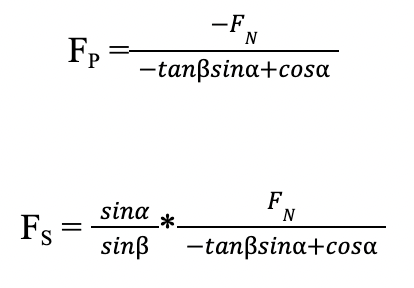
\includegraphics[scale=0.6]{src/figs/legforceequations.png}
\caption{Leg Force Equations}
\label{figs:forceeqn}
\end{figure}

Assuming that the weight of the rocket is distributed evenly amongst the three landing legs, the normal force is equal to (1/3)mg, where m is the total mass of the rocket and g is the acceleration due to gravity. The final mass of the rocket is 3.25 kg, so each landing leg is supporting a normal force equal to 10.63 N. The primary strut is always in compression (negative force) and the secondary strut is in tension. A Matlab script was written that used a nested for loop to cycle through different combinations of $\alpha$ and $\beta$ to find when the summed force was the lowest (the minimum angles for Fp + Fs). The mesh plots can be found in Figures \ref{figs:ml1}, \ref{figs:ml2}.

\begin{figure}[H]
\centering
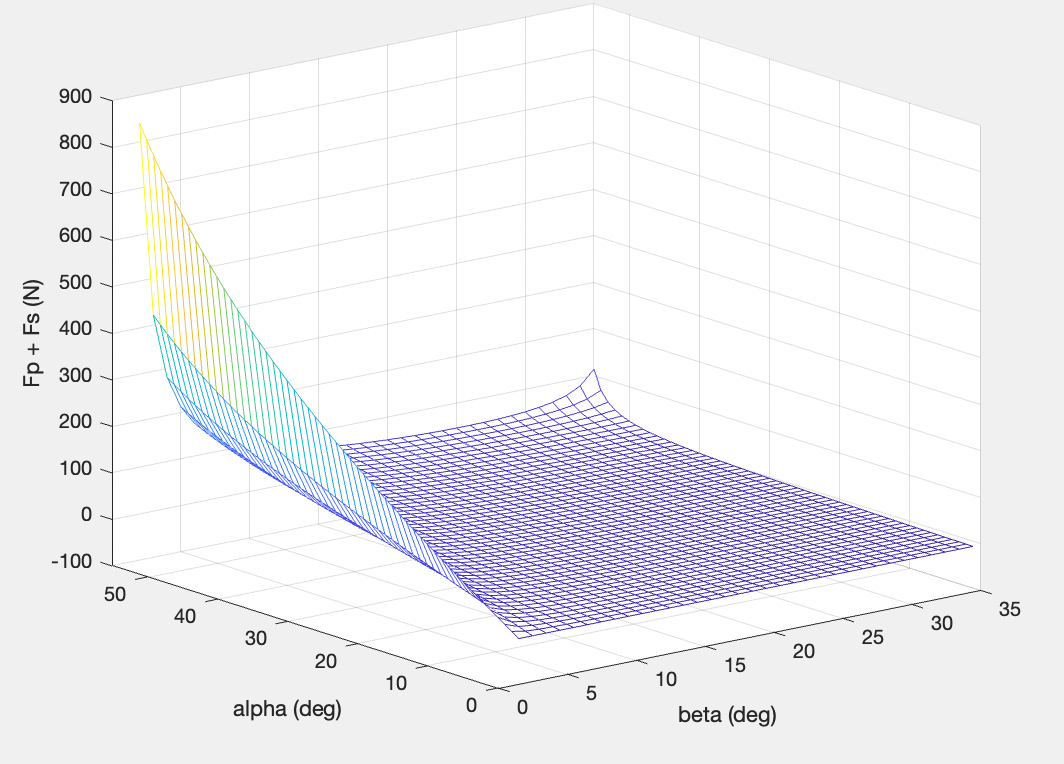
\includegraphics[scale=0.6]{src/figs/ml1.png}
\caption{Matlab Results: Internal force in Legs}
\label{figs:ml1}
\end{figure}

\begin{figure}[H]
\centering
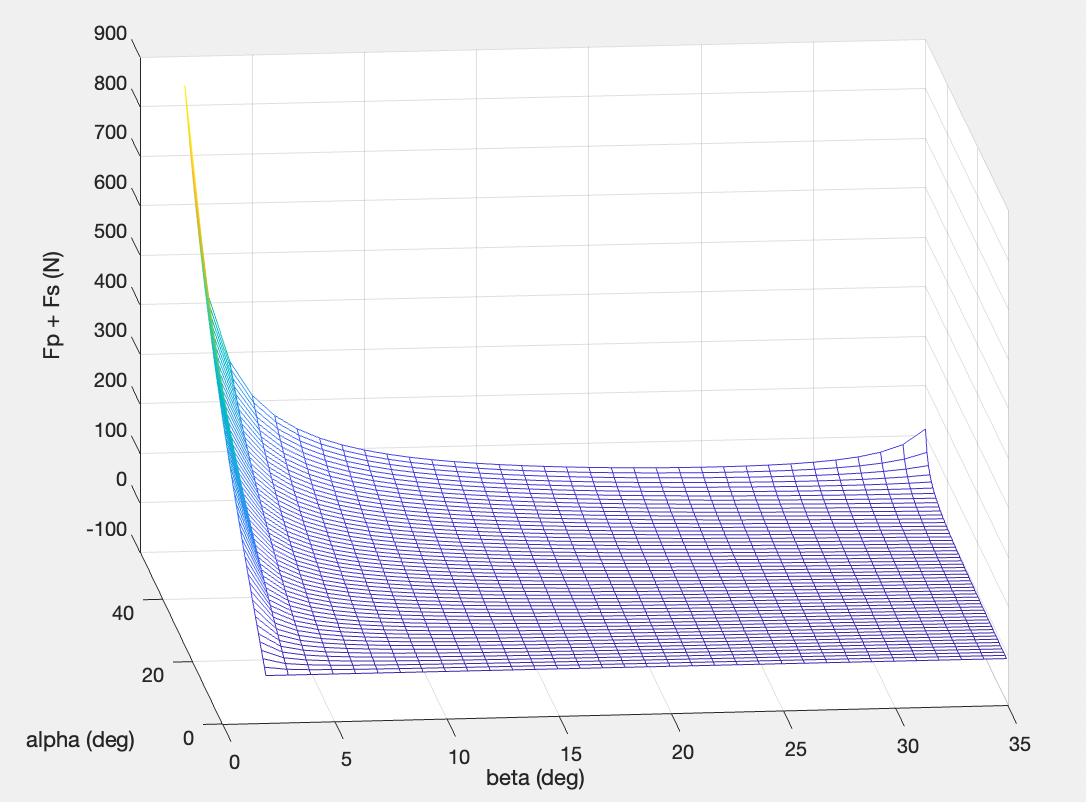
\includegraphics[scale=0.6]{src/figs/ml2.png}
\caption{Matlab Results: Internal force in Legs}
\label{figs:ml2}
\end{figure}

Additionally, the mesh plots in Figure \ref{figs:fpml}, \ref{figs:fsml} display the internal forces in both the primary and secondary strut, respectively. 

\begin{figure}[H]
\centering
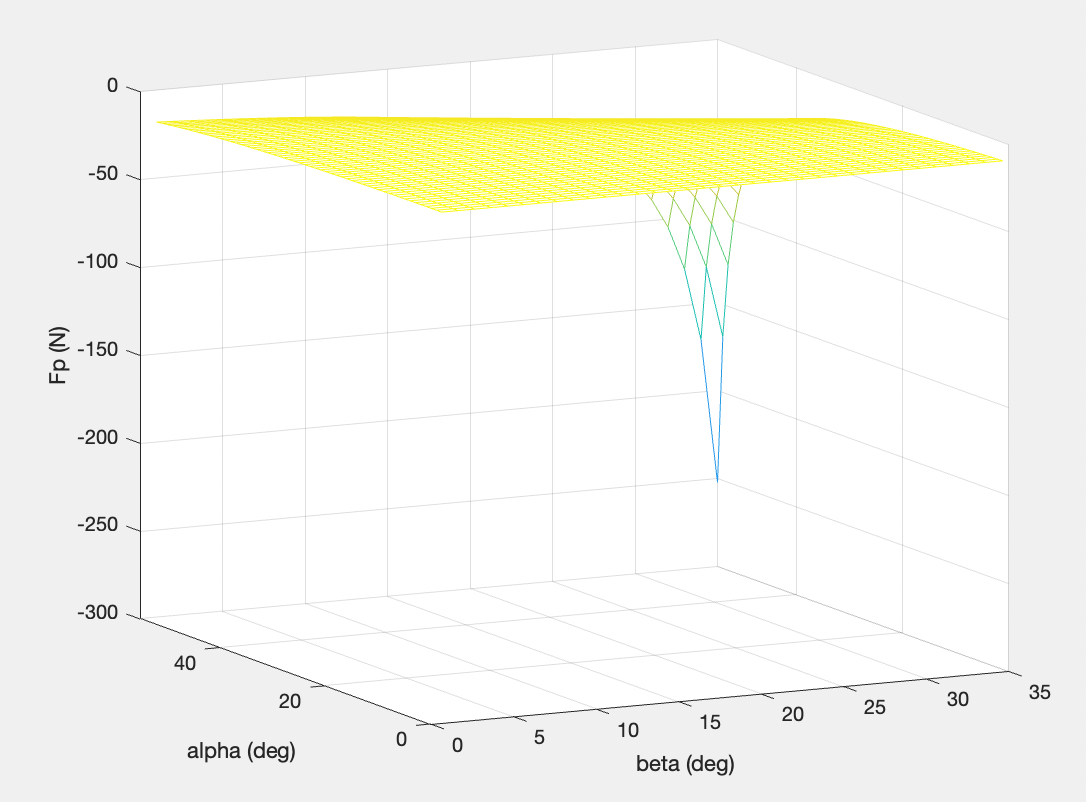
\includegraphics[scale=0.6]{src/figs/fpml.png}
\caption{Matlab Results: Primary Strut Internal Force}
\label{figs:fpml}
\end{figure}

\begin{figure}[H]
\centering
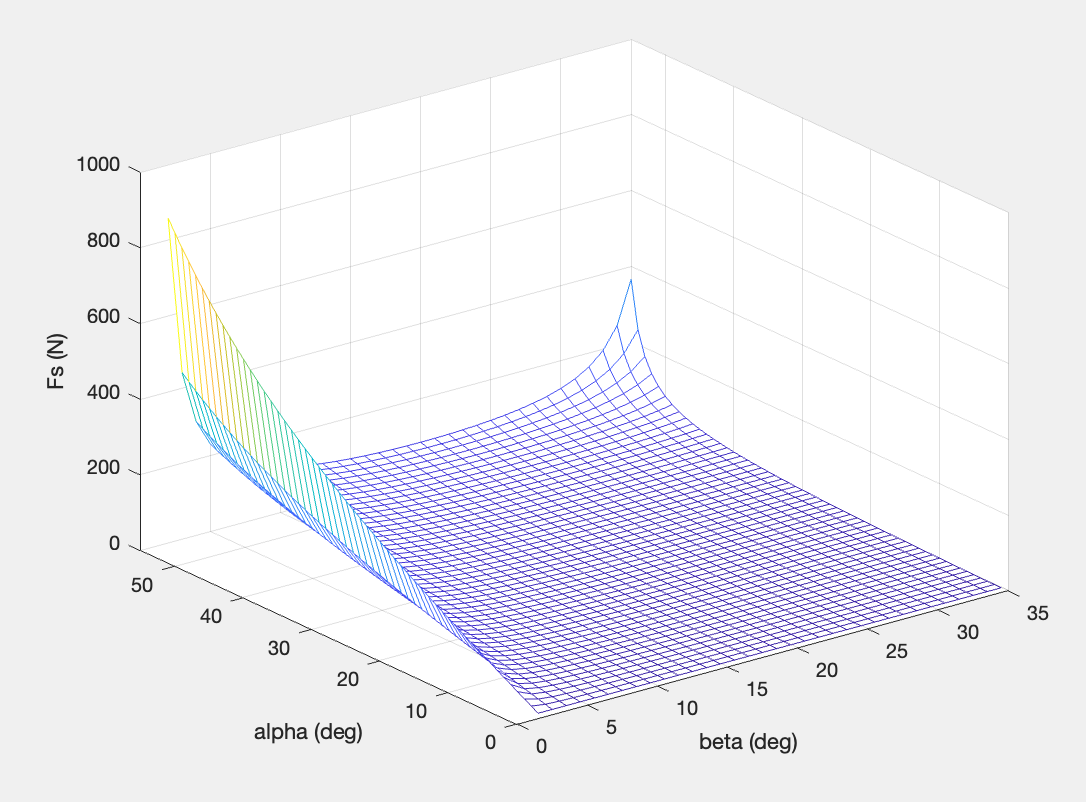
\includegraphics[scale=0.6]{src/figs/fsml.png}
\caption{Matlab Results: Secondary Strut Internal Force}
\label{figs:fsml}
\end{figure}

The primary strut internal force is the opposite sign of the internal force in the secondary strut. Alpha = 19.5 degrees and beta = 45 degrees in the first design iteration. The findings from this analysis suggest that the primary strut is in compression and the secondary strut is in tension based on the angles of the first design iteration of the landing leg assembly. As beta decreases, the magnitude of the internal force of the primary strut decreases and the magnitude of the internal force of the secondary strut increases.  Note that some of these angle combinations do not make sense according to Euclidean geometry and could be another reason why these spikes occur. The locations where the forces are at intermediate are located in the mid-regions of both $\alpha$ and $\beta$. The functional prototype used $\alpha$ = 45 degrees and $\beta$ = 19.5 degrees. After this analysis, these values were maintained because their forces were verified and the footprint was large enough to support a small angled landing while minimizing mass. 

With $\alpha$ = 45 degrees and $\beta$ = 19.5 degrees, Fp = -22.13 N and Fs = 47.23 N. Because the primary and secondary struts are subject to a bending moment, the maximum stress needs to be estimated. 

The stress in each strut can be calculated by using the pinned-pinned model of a beam. The perpendicular force on the primary strut is F = Fn*sin($\beta$) = 10.63*sin(19.5) = 3.54 N, where Fn is the normal force acting on one leg. The moment taken about the point P is equal to 3.54 N * Lprimary = 0.71 Nm. 
The maximum bending stress can be found by using the equation shown in Equation \ref{eq:buckling}.

% \begin{figure}[H]
% \centering
% 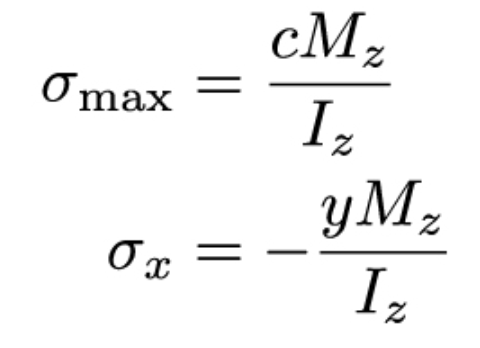
\includegraphics[scale=0.6]{src/figs/buckling.png}
% \caption{Bending Stress Equations}
% \label{figs:buckling}
% \end{figure}

\begin{equation}
    \label{eq:buckling}
    \begin{split}
        \sigma_{max} &= \frac{c M_z}{I_z} \\[5pt]
        \sigma_x &= -\frac{y M_z}{I_z}
    \end{split}
\end{equation}

The c value is the thickness of the primary strut divided by 2, c = 0.0037 m. The moment of inertia about the bending axis is I = 7.26e-10 $m^4$. The maximum bending stress on the primary strut is 3.62 MPa. The strength of the alpha prototype parts is equivalent to carbon fiber, E = 228 GPa. Therefore the primary strut is well over-designed even with a non-zero landing velocity. The maximum bending stress on the secondary strut using the same methodology is Fn*cos(45)*0.1524*0.0037/7.26e-10 = 5.84 MPa. Again, our materials strength surpasses this value and the legs can be reduced in size to further minimize mass. Due to time constraints the team did not redesign and re-manufacture the legs.   